\addcontentsline{toc}{chapter}{Introduction}
\chapter*{Introduction}
Knowing the Earth's topography is crucial for modern geosciences. Different models exist depending on the level of details needed: Earth ellipsoid, its geoid (gravity equipotential surface), contour lines on hiking maps \etc As such, \acrfull{dsm}, which are a representation of a surface's elevation on a regular grid, appear as a natural solution in many \acrfull{gis}. Indeed, they can easily be handled and provide georeferenced information regarding the topography of an area. Figure \ref{fig:intro_dsm_example} presents an example of a DSM. \acrshort{dsm} find usage in various contexts for a wide range of applications. In \acrfull{eo} for instance, \acrshort{dsm} are used to monitor changes in vegetation \cite{sadeghi_canopy_2016}, melting rates of glaciers \cite{berthier_glacier_2014, rieg_pleiades_2018}, volcanos \cite{ganci_data_2022}, snow or water resources \cite{marti_mapping_2016, yamazaki_merit_2019} \etc Similarly, \acrshort{dsm} are employed for catastrophe management, to predict the potential damage caused by earthquakes or floods \cite{jenkins_physics-based_2023} \dots \acrshort{dsm} are also crucial for ortho-rectifying image, \ie geometrically correcting the effects of distortions between the sensor and the terrain. This process creates a planimetric image with a consistent scale in all parts of the image. It allows images to be easily used in GIS or as background for maps. In urban settings, high resolution \acrshort{dsm} can help drone navigation for Defense applications, or more broadly for urban planning \cite{velazco_3d_2012}.

\begin{figure}
    \centering
    \begin{subfigure}[t]{0.5\linewidth}
        \centering
        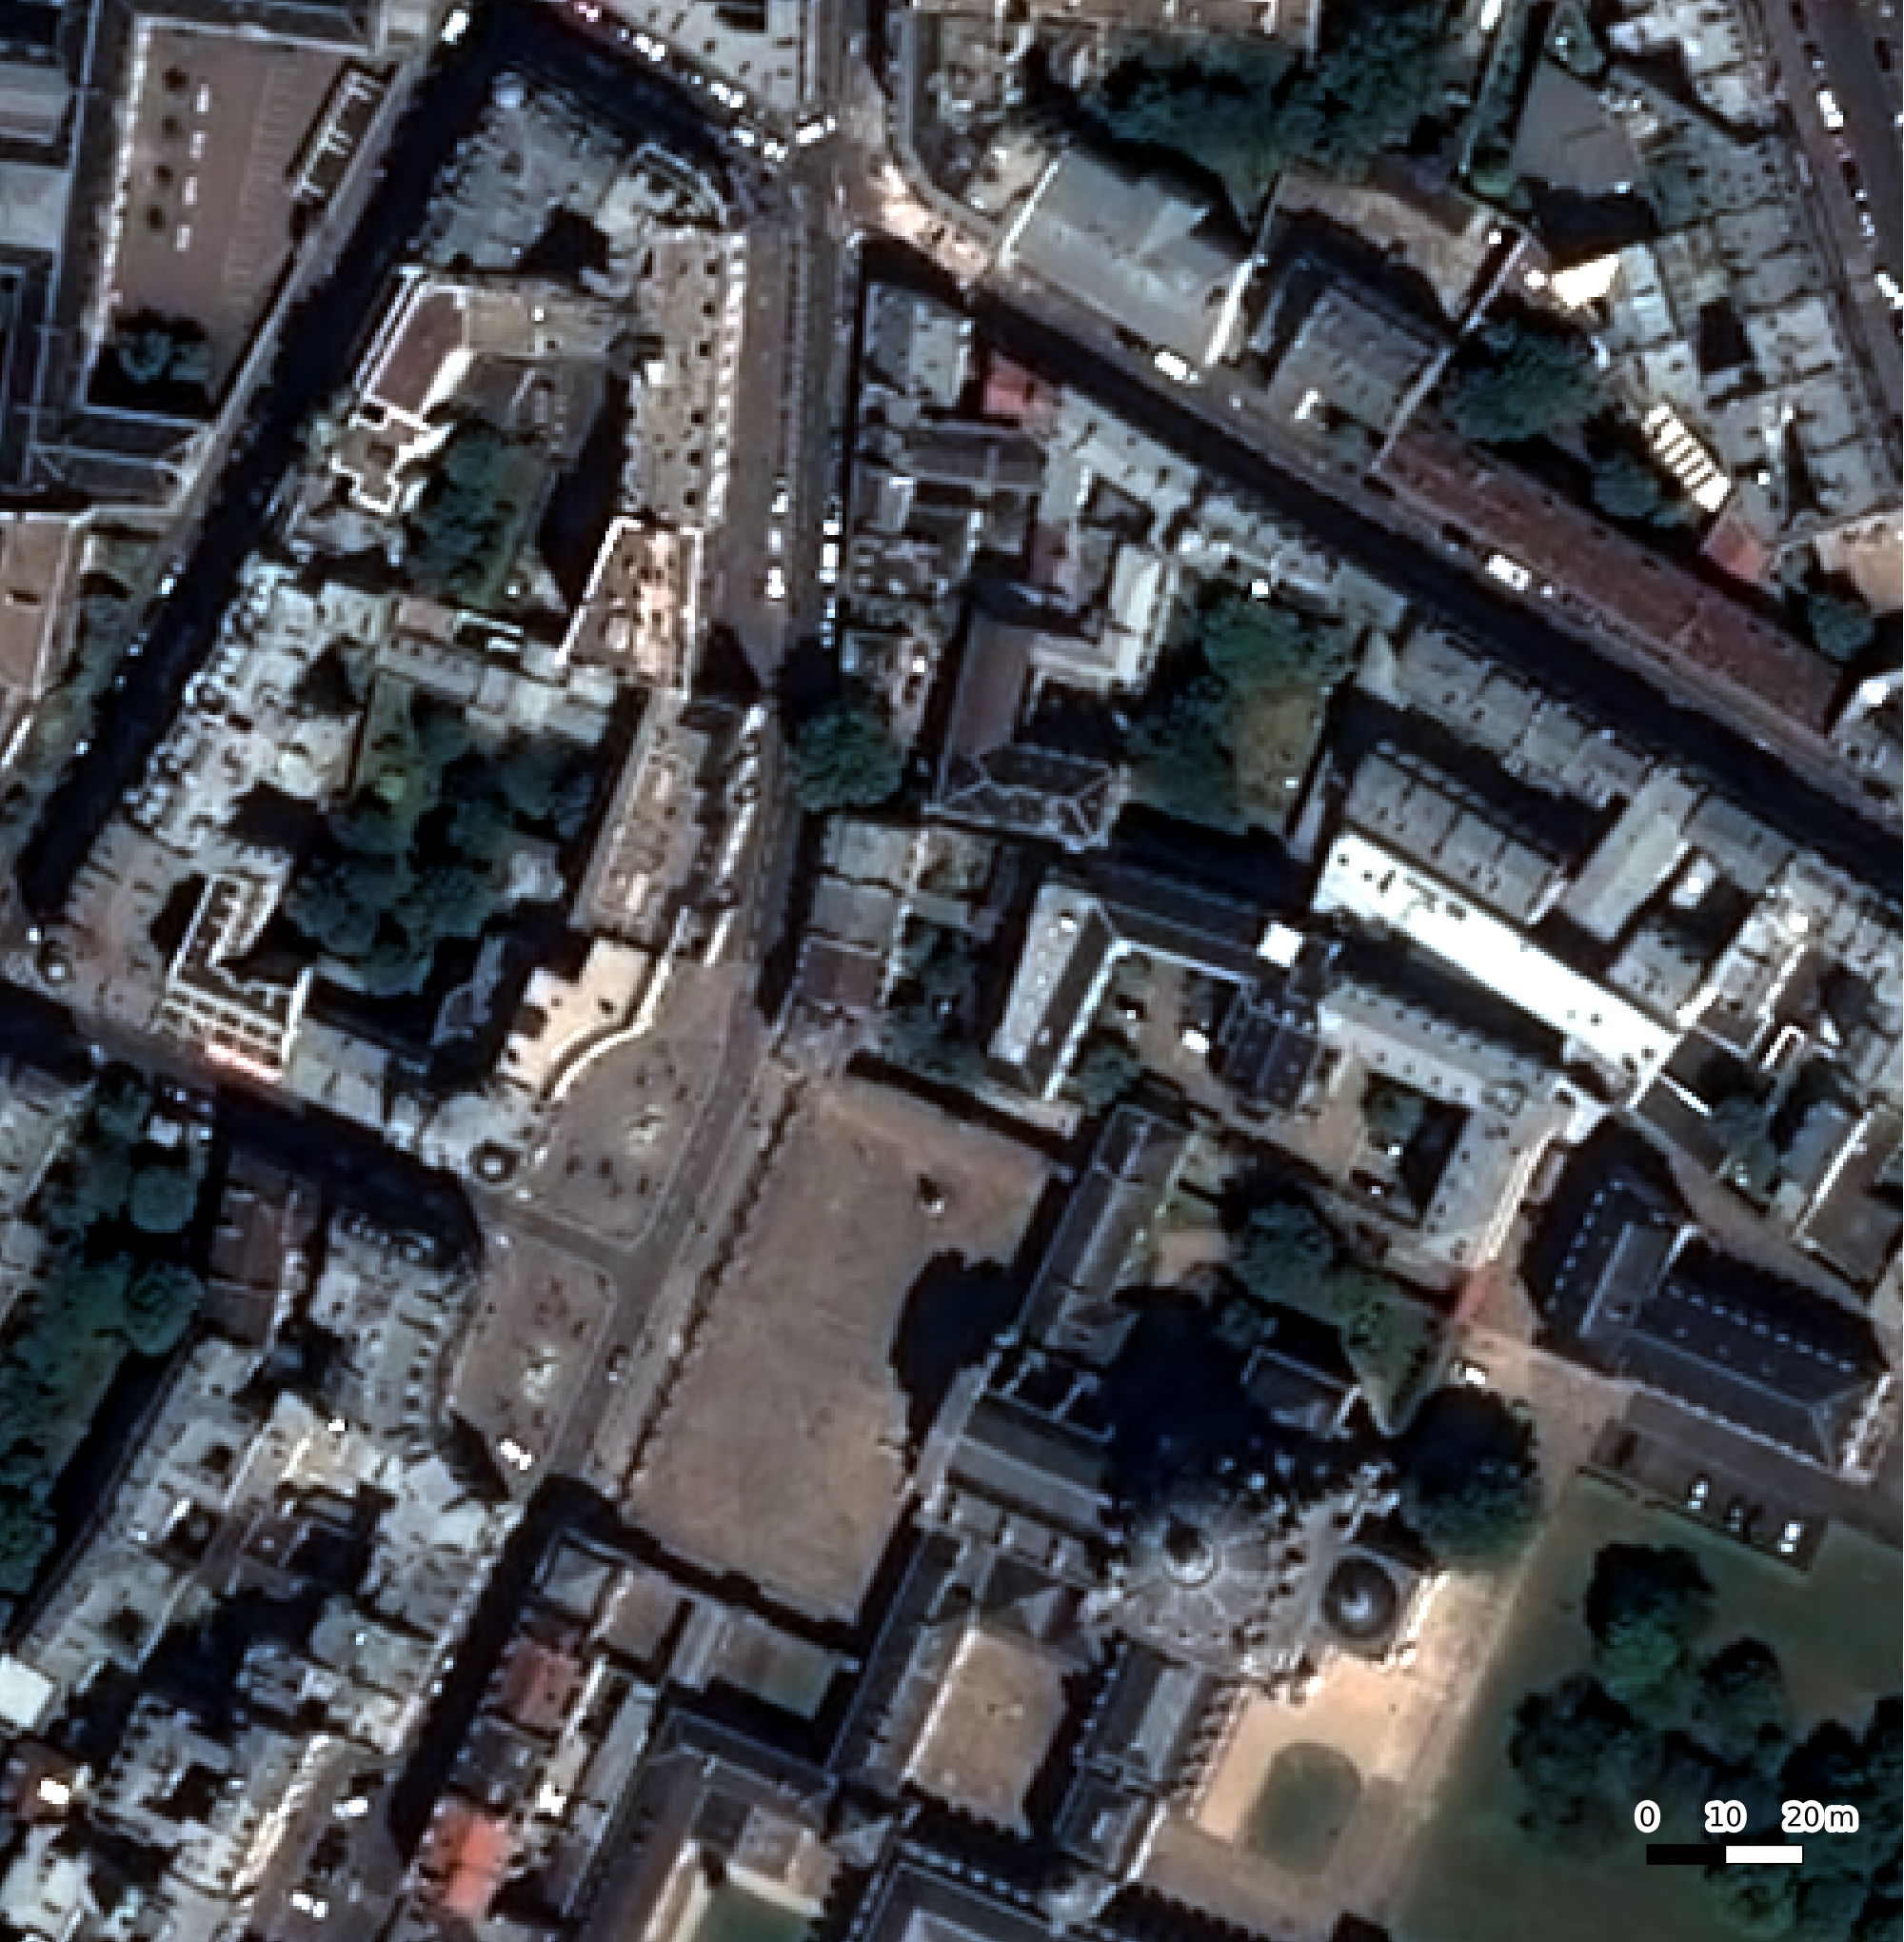
\includegraphics[height=6cm]{Images/0_Intro/Paris_Ortho.png}
        \caption{Pléiades image \copyright CNES 2017, Distribution AIRBUS DS}
        \label{fig:VDG_ortho}
    \end{subfigure}\hfill
    \begin{subfigure}[t]{0.5\linewidth}
        \centering
        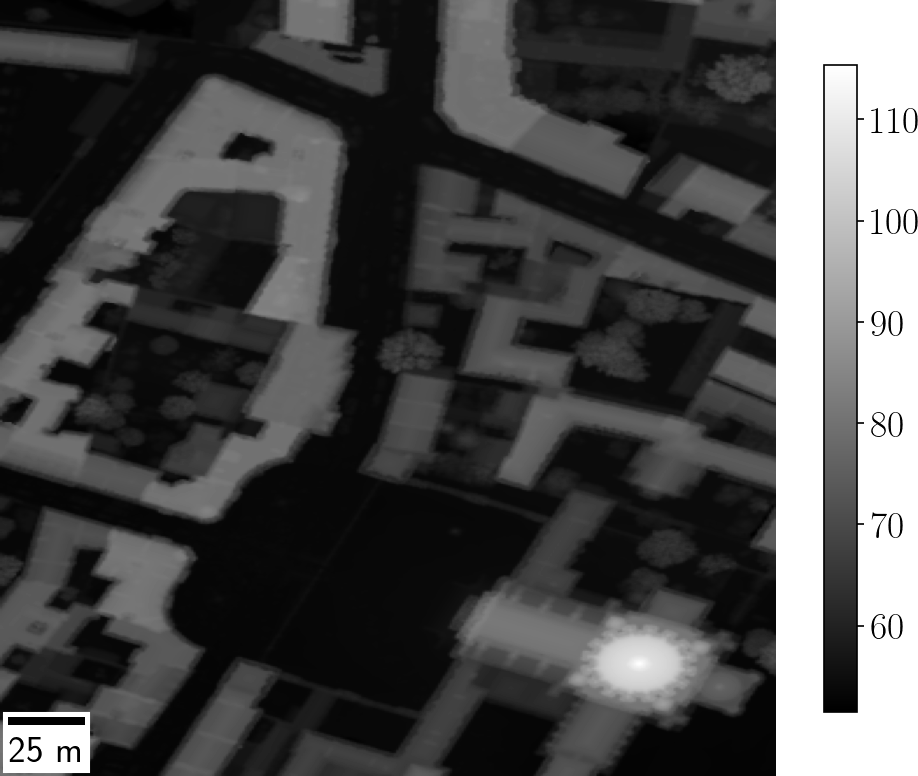
\includegraphics[height=6cm]{Images/0_Intro/Paris_DSM.png}
        \caption{Digital Surface Model from LiDAR HD}
        \label{fig:VDG_dsm}
    \end{subfigure}
    \caption{Satellite image over Val-de-Grâce, Paris at $0.5$m of resolution, and a DSM over the same area.}
    \label{fig:intro_dsm_example}
\end{figure}

There are multiple ways of creating a DSM. Using radar interferometry \cite{farr_shuttle_2007}, LiDAR \cite{khosravipour_generating_2016} or photogrammetry \cite{tao_comprehensive_2001}, each method possessing its own strengths and disadvantages. In this context, CNES - the French Space Agency - is planning to launch 4 optical satellites with Airbus Defense and Space, in order to perform stereo photogrammetry. This mission, named CO3D (for \textit{Constellation Optique 3D}, \cite{melet_co3d_2020}), was conceived jointly with IGN (\textit{Institut national de l'information Géographique et forestière}) to provide high resolution DSM over the globe. CNES also developed a pipeline to process all images provided by the CO3D satellites automatically and at a very large scale. The main objective of this thesis was to characterize and propagate the uncertainty amongst this photogrammetry pipeline.

\commanue{Bonne intro sur l'incertitude, bravo ! Il te faudrait une petite phrase ou deux de transitions sur pourquoi tu abordes maintenant l'incertitude}
As we will deal with uncertainty throughout this thesis, we first need to specify what we mean by uncertainty. Uncertainty is a situation where a measure or value of interest is not known, or not known with precision. It is subject to change, as additional information, measures or a different acquisition protocol may reduce how uncertain a value is. It can also be subjective. For instance someone maybe uncertain about the launch date of CO3D satellites while someone else working at the launch pad might have the answer. This highlights the fact that while everyone has an understanding of what uncertainty is, it encompasses very different concepts in nature. It is common to differentiate the various types of uncertainty by dividing it into two categories: stochastic (or random) uncertainty and epistemic uncertainty.

Stochastic uncertainty refers to every situation of purely aleatoric nature. For instance, the result of a coin throw, random noise on a CCD captor or the Brownian movement of a particle. An operator typically encounters this kind of uncertainty in a situation where they have access to many measures or observations of the same value of interest. It is usually modeled mathematically with a frequentist approach, using probability measures such as the uniform distribution, Gaussian distribution, Student's $t$ distribution \etc 

On the other hand, epistemic uncertainty refers to a situation where the value of interest is not known or ill-known due to a lack of knowledge. Think of the previous example with the launch date of satellites, or if someone was asked to guess Io's mass, one of the moons of Jupiter. There is no random process at stake here, and there is usually no point of acquiring multiple samples of the measure. Once the value of interest is known, the uncertainty usually no longer exists. It has been proposed to model this kind of uncertainty using a Bayesian approach for probability, by opposition with the frequentist approach. Probabilities here represent a state of knowledge, or degree of belief, one has over the value of interest. It can be update with additional knowledge, thus leading to the notion of prior and posterior probabilities. We will see during this thesis that other model can be used to characterize this uncertainty. 

Although uncertainty can be complex and expensive to compute, characterizing and quantifying it has many benefits. It provides additional information for better decision making and risk management. It can also allow for a better understanding of the underlying processes at stake regarding the value of interest. In many cases, uncertainty estimation is treated as a secondary objective in applications. However, jointly estimating a value and its uncertainty can lead to new strategies to reduce the uncertainty or sometimes even improve the performances of the main applications \cite{chen_learning_2023,jiang_unsupervised_2024}.

The objective of this thesis is to investigate methods for estimating and propagating the uncertainty in a stereo pipeline. In the context of this thesis, we focused mainly on a pipeline developed by CNES, called CARS, which will be used for a mission dedicated to stereo-photogrammetry called CO3D. 

During this thesis, we both contributed to the field of \textit{imprecise probabilities} (a specific type of uncertainty model) \cite{}, to the dielcomputer vision 
in section \ref{sec:different_models_of_uncertainty}

The following publications:
National conferences:
\begin{itemize}
    \item Rencontres francophones sur la logique floue et ses applications (LFA 2022) - \cite{malinowski_copules_2022}
\end{itemize}
International conferences:
\begin{itemize}
    \item 10th International Conference on Soft Methods in Probability and Statistics (SMPS 2022) - \cite{malinowski_copulas_2022}
    \item 13th International Symposium on Imprecise Probabilities: Theories and Applications (ISIPTA 2023) - \cite{malinowski_uncertainty_2023}
    \item 2024 IEEE International Geoscience and Remote Sensing Symposium (IGARSS 2024) - \cite{malinowski_robust_2024}
\end{itemize}
International journals:
\begin{itemize}
    \item Go to journal home page - International Journal of Approximate Reasoning
International Journal of Approximate Reasoning (IJAR) - \cite{malinowski_uncertainty_2024}
\end{itemize}

The follwoing pre-print is not yet published:
\begin{itemize}
    \item \cite{malinowski_robust_2024-1}
\end{itemize}
\todoroman{Propisition: contexte, objectif, contributions, contenu de la thèse, papiers, séminaire ausquels j'ai participé}
\todoroman{Mettre un reading guide pour dire quel ``niveau d'expertise'' il faut en fonction des chapitres }
\todoroman{Scope of this PhD}
\todoroman{Une image pléiade et son LiDAR HD ?}
\pagebreak